\chapter{Methods}

\begin{comment}
\section{{Protocol:First Part}
\begin{itemize}
\item 5 jumps
\item lie down on \textbf{prone} position
\item 5 jumps
\item lie down on \textbf{left side} position
\item 5 jumps
\item lie down on \textbf{supine} position
\item 5 jumps
\item lie down on \textbf{right side} position
\end{itemize}


\section{Data Collection Protocol}





The aim of this protocol is to collect data with the two mattresses (SensigTex under the Sensomative) of different heart rates and breath rates.
During this protocol will be asked to change positions to collect the data in all four positions: supine position, lateral right position, prone position, and lateral left position.
Before data collection will also record what the sensors measure in case a participant is not on the mattress whether it is stationary or moving.




\section{Experimental Setting}
The experimental setting includes a bed above which two sensors will be positioned: SensingTex and Sensomative. The Sensomative has to be placed under the  SensingTex Sensor and the sensor will be used simultaneously. 
\subsection{Mattress }
The Sensomative Sensor gives the best result for detecting breath rate and heart rate when placed under the chest.[\textbf{investigate possible distance from the start of the mattress}] For this reason, should be placed exactly []cm from the top part of the mattress.
Above this sensor, the SensingTex Sensor should be placed above this sensor because applying even pressure will not affect the measurements.
\subsection{Pillow and bed sheets}

\subsection{Ground truth }
The ground truth value for this data collection will be collected via polysomnography and video cameras. Polysomnography allows to recording this following parameters:

\begin{itemize}
    \item Nasal flow and nasal pressure: that will be used as the ground truth for the breath rate.
    \item Chest and abdomen movement: that can be also used as ground truth for the breath rate, with different types of approaches. [\textbf{can also detect the heart rate o heart movement?}]
    \item SPO2 and Pulse with a fingertip: that will be the ground truth data for the heart rate
    \item \{ Raimon \} 
\end{itemize}

Along with Polysomnography will also be involved cameras to record the position of the participant for further analysis.

\section{Patient setting}
\subsection{what to wear}
The participant should wear comfortable clothes. T-shirts are recommended in order not to have a too high layer of fabric that could interfere with the detection of data, in particular with the heart bit detection.
\subsection{Lay down position}
There are four different positions that will be asked to\begin{itemize}
    \item Lateral left position
    \item Lateral right position
    \item Prone
    \item Supine
\end{itemize}
\subsection{Pattern Position}
One of this data collection's main points is finding peaks in different positions, so each patient will be asked to lay down in a different position pattern.
\begin{itemize}
    \item supine position, lateral right position, prone position, and lateral left position
    \item lateral right position, prone position, lateral left position and supine position
    \item prone position, lateral left position, supine position and lateral right position
    \item lateral left position, supine position, lateral right position and prone position
\end{itemize}
Once a position pattern is given to a specific participant, it must be repeated for each step of the protocol.
\subsection{how long they have to lay down}





\section{Data Collection}
\subsection{Joint Data Collection}
\subsubsection{Breathing rate and Heart rate at rest in normal condition}
In this part of the protocol, the aim is to collect data on the breathing rate and heart rate of the participants at rest.
\subsubsection{Breathing rate and Heart rate at rest during mattress movement}
This part of the protocol aims to collect data on the participant's breathing rate and heart rate at rest while the mattress is moving.
\subsubsection{Breathing rate and Heart rate after an effort}
In this part of the protocol, the aim is to collect data on the participant's breathing rate and heart rate after an effort, to analyze data of an accelerated breath and heart bit and gradually decelerated.
The effort consisted of ten jumping jacks repeated before each position change.

%\section*{Breath Rate}



\subsection{Heart Rate Data Collection}
\subsubsection{Heart rate at rest with constrained breath rate}
This part of the protocol aims to provide a known rhythm to the breath rate according to an acoustic time. The sound will indicate when they start to inhale and exhale to the participants.

\subsubsection{Heart rate at rest with constrained breath rate during mattress movement}
This part of the protocol aims to provide a known rhythm to the breath rate according to an acoustic time while the mattress is moving. The sound will indicate when they start to inhale and exhale to the participants.

\end{comment}

%%%%% INSTRUMENT %%%%%

\section{Instruments}
The project involved two textile sensor mattresses: Sensomative and SensingTex (described in Chapter \ref{cap:SensomativePar} - \ref{cap:SensigTexPar}) and a rocking bed Somnomat Casa described in Chapter \ref{cap:Somnomat}.

The chosen instrument to collect the ground truth, cardiopulmonary polysomnography, is Nox A1, described in Chapter \ref{cap:NOXA1}.

%%%%% SENSOMATIVE %%%%%

\subsection{Sensomative}\label{cap:SensomativePar}
Sensomative (Rothenburg, Switzerland)\cite{sensomativeUrl} is a start-up company, founded in 2015 in Switzerland, which produces textile pressure-measuring mats. These are based on the same principle as resistive touchpads. The sensor mass
consists of two layers of conductive textile which are separated from each other by a spacer grid. 

The sensor seen in Fig.\ref{fig:sensomativeBed} is composed of 14 x 28 sensor elements with a sampling frequency of 50Hz. 
The sensing area is 40 cm x 80 cm and thus stretches almost over the entire width of a standard-sized bed. Each sensor element is round and has a diameter of 2 cm.
This mattress is commonly used to investigate position since is possible to have the pressure distribution (example visible in Fig.\ref{fig:sensomativeData}). This mattress is used, for example, to control the sitting posture of office chairs and wheelchairs, analysing the pressure distribution is possible to discover posture errors and uneven loads.\\

\vspace*{0.5cm}
\begin{figure}[H]
    \centering
    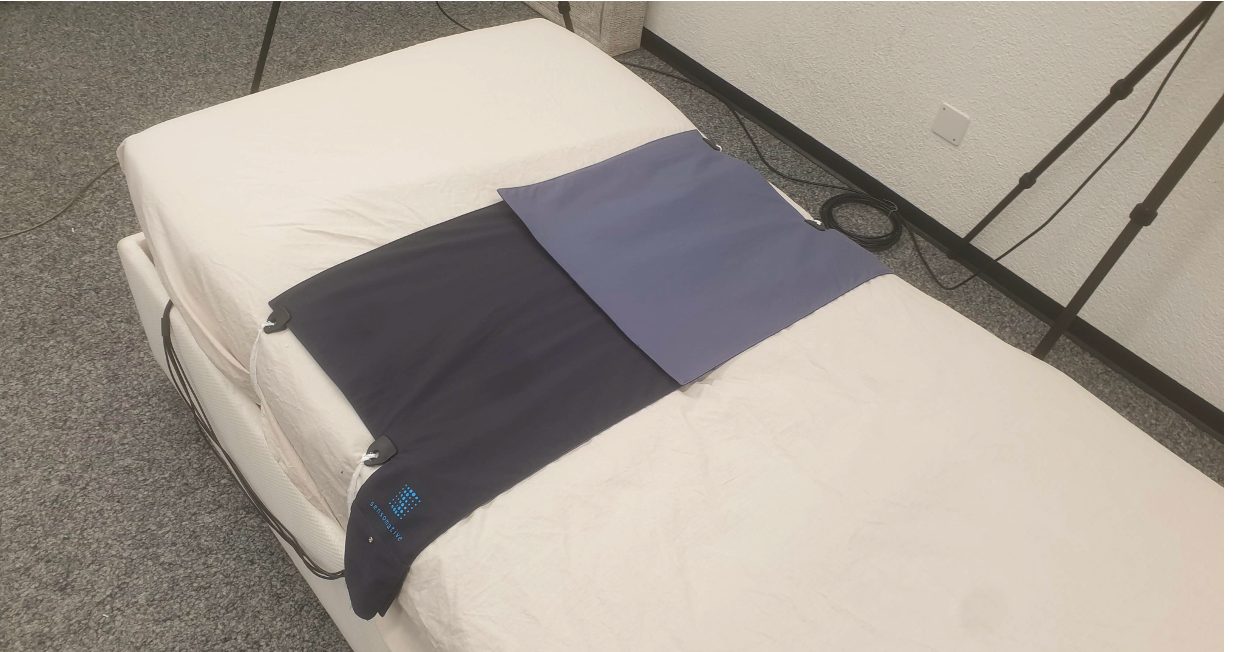
\includegraphics[width=0.9\textwidth]{img/sensomative.png}
    \caption{Sensomative over a bed}
    \label{fig:sensomativeBed}
\end{figure}
\vspace*{0.5cm}

However, its dimension of 40 cm x 80 cm does not allow it to cover the entire mattress so it is crucial to find the correct position to detect the desirable data. In this project, the aim is to estimate the respiration rate so the position chosen is under the lungs, so from just above the shoulder to the middle of the abdomen.

This is to be able to track the movement of the thorax during respiration. The movement is extracted and evaluated from the single sensor channel of the mattress, for the inhalation phase it has been seen an increase in pressure and during the exhalation phase a decrease. Following a pattern [DATA] similar to nasal pressure or RIP Flow, recorded by the cardiopulmonary polysomnography \ref{cap:NOXA1}. 

The data for this mattress are a subsection of the entire data and come from a previous data collection of one of the supervisors of this thesis, Manul Fujis \cite{ManuelZurich}, who kindly make them available to inspect further the possibility to estimate respiratory rate from this mattress and also to have the data to do a preliminary study of the general feasibility to extract this physiological data. 



\begin{figure}[H]
    \centering
    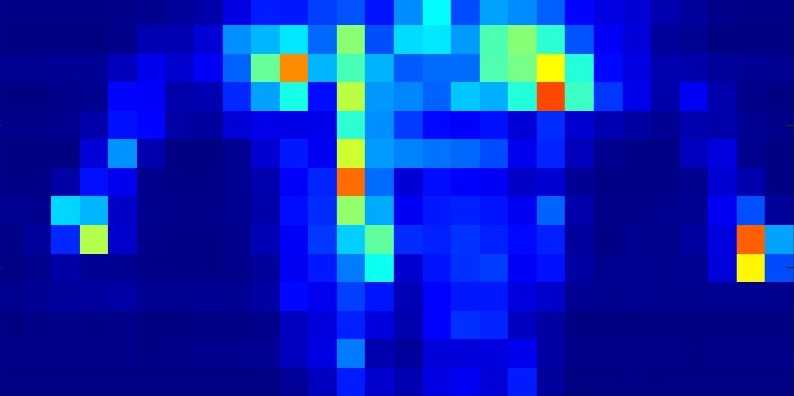
\includegraphics[width=0.9\textwidth]{img/sensomative_2.jpg}
    \caption{Sensomative data}
    \label{fig:sensomativeData}
\end{figure}
\vspace*{0.5cm}

%%%%% SENSINGTEX %%%%%
\subsection{SensingTex} \label{cap:SensigTexPar}
The instrument on which this thesis is focalised then is SensigTex \cite{SensingConnectivity}, visible in Fig \ref{fig:sensingtex} this is a commercially available textile pressure sensor mattress. 
The Mattress Mat Dev Kit is capable to cover the entire area of a bed measuring 192cm x 94cm, with 48 x 22 sensor elements and a sampling rate of 10Hz. This means that is five times slower than Sensomative (Chapter \ref{cap:SensomativePar}), but that is already installed in a hospital ward of the \textit{University of Bern} for the study research on movement disorders during sleep in patients with Parkinson's disease. The ability to estimate breath could be helpful for that study and then this project focused on this possibility.

This mattress is already implemented in the context of position classification because as shown in Figure \ref{fig:sensingtexData}, is possible to retrieve the position of the person on it. The raw data has a scale in the range of 0-256 (minimum-maximum). 

Looking closer into signals of singles channels is possible to see a pattern that resembles a breathing rhythm,  similar to the data that can
 be retrieved from the nasal pressure exerted on the cannula of cardiorespiratory polysomnography, as shown in Figure \ref{fig:404}.



\vspace*{0.5cm}
\begin{figure}[H]
    \centering
    \includegraphics[width=\textwidth]{img/sensingTex.png}
    \caption{SensigTex over a bed}
    \label{fig:sensingtex}
\end{figure}

\begin{figure}[p]
    \centering
    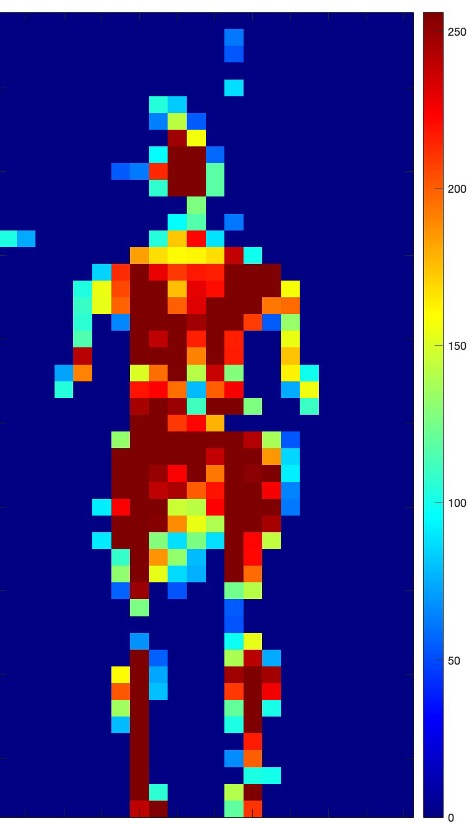
\includegraphics[width=0.7\textwidth]{img/sensingtex_2.jpg}
    \caption{SensigTex Data }
    \label{fig:sensingtexData}
\end{figure}
%\vspace*{0.5cm}

%%%%% NOXA1 %%%%%
\subsection{Nox A1, polysomnography} \label{cap:NOXA1}
As explained in Chapter \ref{cap:cardiorespiratory} cardiopulmonary polysomnography is an accepted method to monitor physiological data during sleep.

Since in the data collection conducted during the thesis, further explained in Chapter \ref{cap:dataCollection}, it has been necessary to have a gold standard to track the respiratory rate and validate estimated respiratory rate from the pipeline, described in Chapter\ref*{cap:pipeline}.

The instrument chosen has been Nox A1 of NoxMedical, shown in Figure \ref{fig:NOXA1}, a wireless and portable PSG recording the following physiological parameters: 

\begin{itemize}
    \item Nasal pressure and Nasal Flow via nasal cannula.
    \item Chest and Abdomen Movement with respiratory inductance plethysmography (RIP) gathered together in a parameter called "RIP Flow"
    \item Heart Rate (ECG)
    \item SPO2 and Pulse with a fingertip
\end{itemize}

In the pipeline (Chapter\ref*{cap:pipeline}) it has been decided to use the Resp Rate (respiratory rate) calculated by the NOX A1 and displayed as respirations per minute or [rpm] based on RIP Flow data.
However, to further understand if the channels in the mattress represent the correct respiratory rate also used Nasal pressure and Nasal Flow.

\begin{figure}[H]
    \centering
    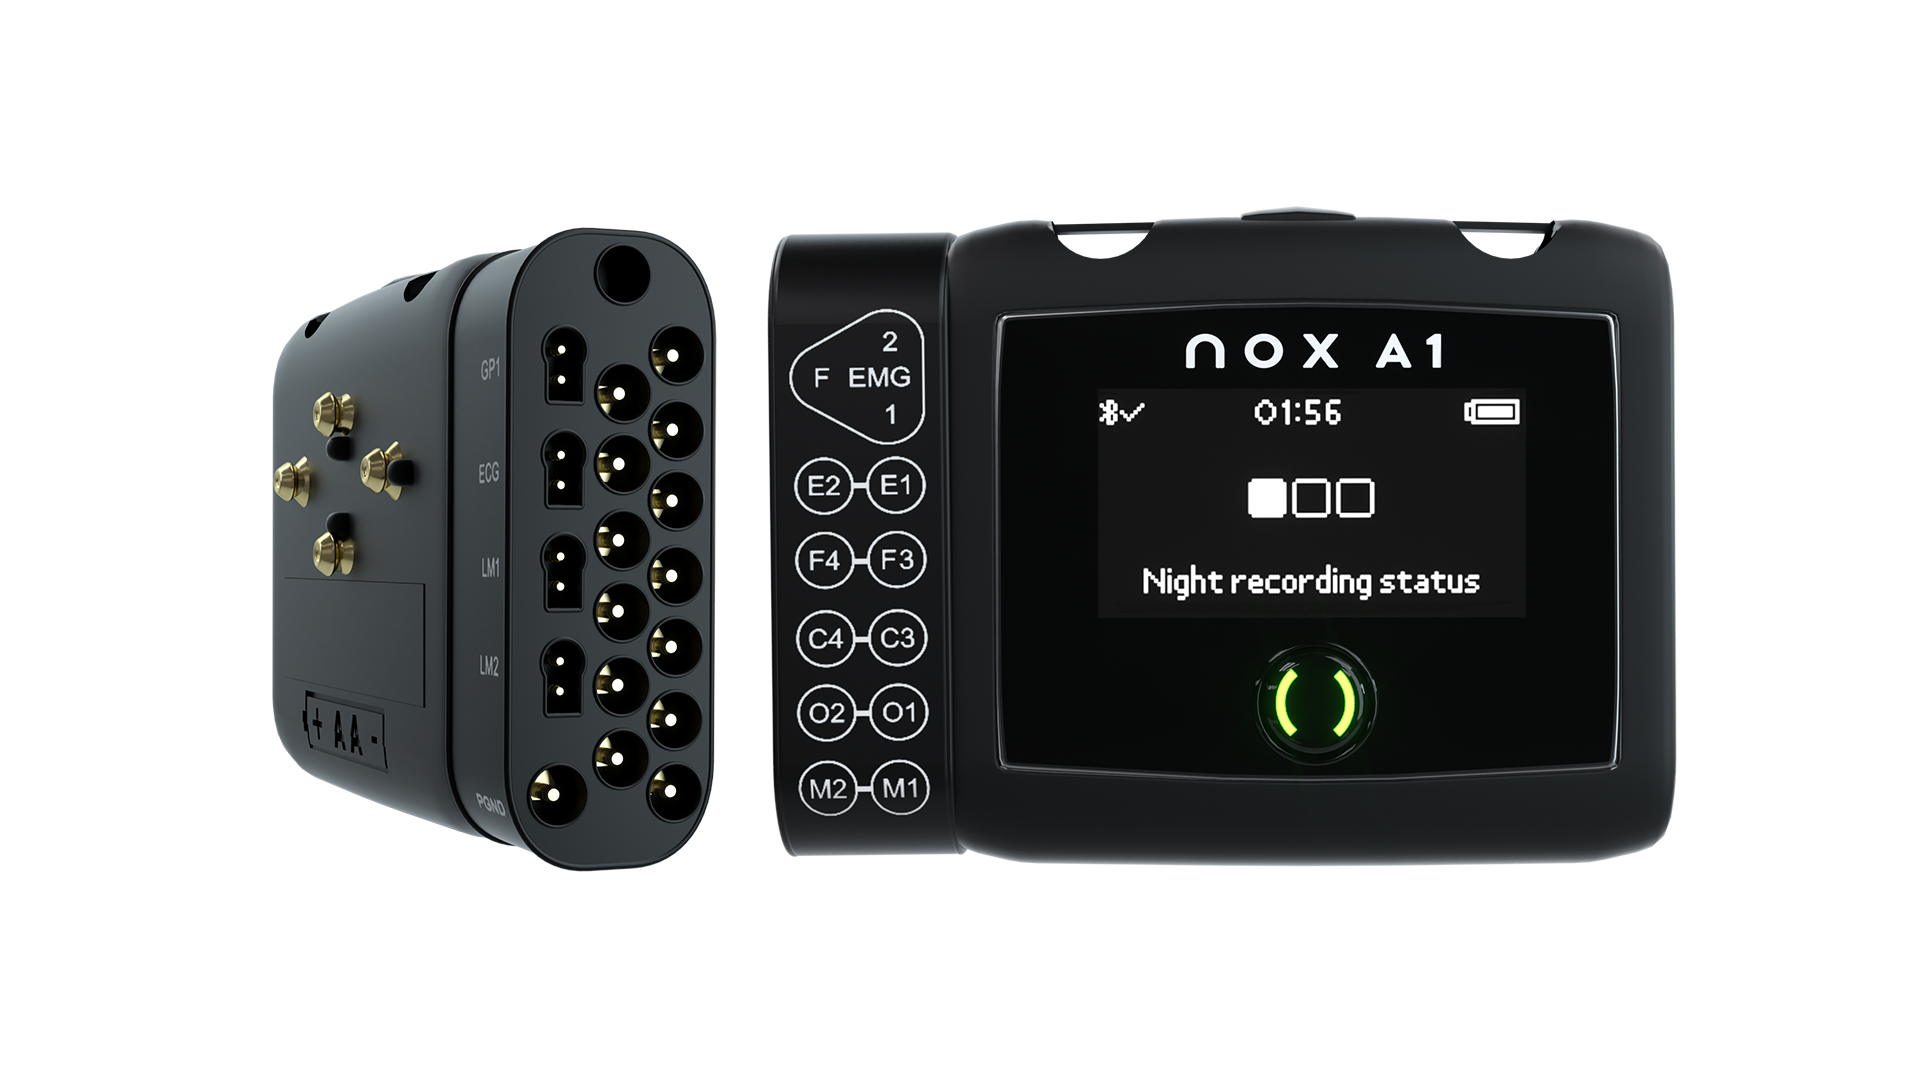
\includegraphics[width=\textwidth]{img/1.png}
    \caption{Nox A1™ PSG System device of NoxMedical}
    \label{fig:NOXA1}
\end{figure}

%%%%% SOMNOMAT %%%%%
\subsection{Somnomat Casa} \label{cap:Somnomat}
The lab, where this thesis is carried out, has one of the main focuses on sleep robotics. Inside the Somnomat project, there are two research domains: one covers controlled positional therapy and the other investigates the potential benefits of rocking movements on sleep.

The second research domain aims to replicate the rocking movement made by the mother to help babies to fall asleep, replicating back-and-forth motions. The Somnomat Casa, shown in Figure\ref{fig:somnomat}, looks like a conventional bed but fits into private bedrooms and can be operated by the push of a button. 
Rocking movement has determined suitable motion parameters and mechanical adaptations to have an inaudible rocking mechanism.

The possibility to estimate the respiratory rate of a person while the rocking bed is moving could be important to discover how this movement could help to fall asleep, based also on the respiration rate. As discussed in Chapter \ref{cap:sleepStages}, breathing is one of the parameters that highlight the sleep stage in which the person is in that moment. This knowledge could be used to further implement the intervention.


\begin{figure}[H]
    \centering
    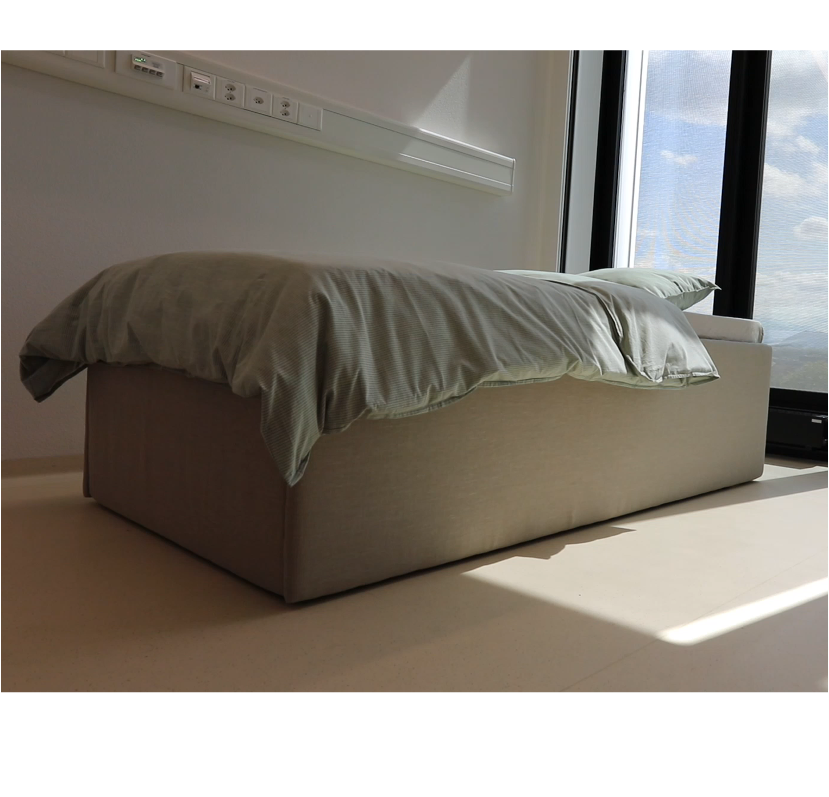
\includegraphics[width=0.8\textwidth]{img/somnomat.png}
    \caption{Somnomat}
    \label{fig:somnomat}
\end{figure}


%%%%% DATA COLLECTION %%%%%
\section{Data Collection} \label{cap:dataCollection}

In the course of the thesis project been conducted data collection because the data from Sensingtex where not has been collected yet.
However, the availability of a rocking bed gives this data collection a second objective.
The primary objective has been to collect data from SensingTex to understand the feasibility of extracting breath rate from the mat; 
the second goal is to understand if the movement of the rocking bed could influence the signal.

The participant involved was 6, half male and half female, between 20-30 years old, who were asked to lie on a standard mattress covered with the sensor mattresses in a specific position, for the first part of the data collection (described in Chapter \ref{cap:NormalBed}), and on a rocking bed while it is moving, for the second part of the data collection (described in Chapter \ref{cap:RockingBed}).
Each participant wore a cardiorespiratory wireless and portable polysomnography device (Nox A1 PSG of Nox Medical), described in Chapter \ref{cap:NOXA1}. The total length of the data collection for each participant is 36 minutes long divided into 4 minutes in each of the 4 positions with normal bed and with Somnomat.

%%%%% NORMAL BED %%%%%
\subsection{Normal Bed}\label{cap:NormalBed}
The first part of the data collection aims to understand the feasibility of extracting breath rate from the mat, so the setting involves the pressure mat over a standard bed.  

During the night and through the different sleep stages, the breath rate increase or decreases, so we decide to insert a similar variability in our data. Since this study is performed in a laboratory condition to recreate this it has been asked to the participant to perform a set of five jumps before lying down, so it is expected to find in the data this variability that is firstly checked with the data coming from the ground truth.

The participant performs the jumps and then lies down on a mattress in a specific position for 4 minutes.
After that, they were asked to stand up, perform the other 4 jumps and go down again. This is done for each of the positions of the pattern: supine left side, prone, and right side. The total number of jumps performed is 20 and the Toal time for this part is about 18 minutes (including getting in and out of bed and jump time).

\begin{figure}[H]
    \centering
    
\includegraphics[width=0.8\textwidth]{img/PLACE HOLDER.pdf}
    \caption{Place holder normal bed}
    \label{fig:normalBed}
\end{figure}

%%%%% ROCKING BED %%%%%
\subsection{Rocking Bed}\label{cap:RockingBed}
The second part of the data collection aims to understand if the movement of the rocking bed could influence the signal.

 Since the data are collected while the Somnomat Casa is moving, it has been fixed the period for the movement of the bed at 4 seconds (15 periods in a minute) with an acceleration of 0.25 $m/s^2$. 
 The participant has not been asked to perform any jumps, to have less variability in breath patterns and see the possible interference from the mattress.
They have been asked to lie down in a supine position for 4 minutes, and after that, they have been asked to turn around on the left side. This has been asked to perform for all the positions: supine, left side, prone, and right side.
The total time for this part is about 18 minutes, including the necessary time to turn around on the bed and stop the movement between each position.


\begin{figure}[H]
    \centering
    
\includegraphics[width=0.8\textwidth]{img/PLACE HOLDER.pdf}
    \caption{Place holder rocking bed}
    \label{fig:rockingBed}
\end{figure}

\subsection{Data processing} \label{cap:dataProcessing}

After the data collection, it has been necessary to clean the data in order to remove the moment when the participant was getting in and out of the bed.\newline

 For each recording, based on different data extracted from the PSG and pressure mattress, is possible to retrieve when the person stands up to perform the jumps or to turn around in another position. As shown in Figure \ref{fig:recordingCutfull}, based on nasal pressure data, is possible to recognize the different moments. In the left part of the plot the four positions on the stationary bed and in the right part the four positions on the moving bed.
 In the end, for each participant are available eight different recordings, 4 minutes long, one for each position of the different phases in which the data collection is divided.


\begin{figure}[H]
    \centering
    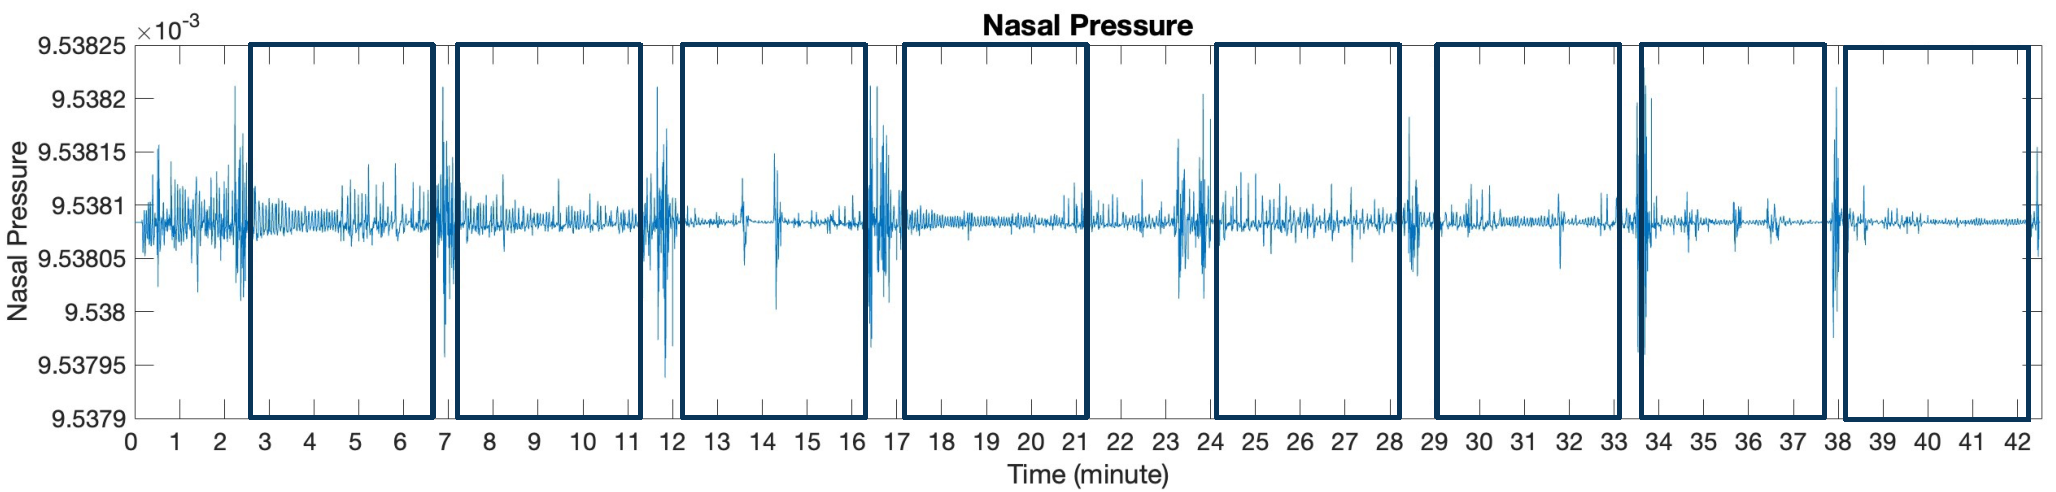
\includegraphics[width=\textwidth]{img/full_new.pdf}
    \caption{Full recording of a participant - 42 minutes long}
    \label{fig:recordingCutfull}
\end{figure}